\documentclass[10pt]{article}
\usepackage[margin=0.75in]{geometry}
\usepackage{tikz}
\usepackage{amsmath}
\usepackage{enumitem}
\usepackage{color,soul}

\usepackage{multicol}

\newcommand{\ds}{\displaystyle}

\begin{document}
\newcounter{enumCount}
\pagestyle{empty}
\subsection*{Math 105 - Homework 6 \hfill Name: \underline{\hspace*{2in}}}
\textit{Solve the following without using a calculator.}

\noindent
\begin{enumerate}


\item If $f(x) = 5+x$ and $g(x) = \sqrt{x}$, then what are $f(g(4))$ and $g(f(4))$? 
\vfill

\item Suppose $f(x) = x^2-4$ and $g(x) = 2-3x$.  How far apart are $f(3)$ and $g(3)$ on a number line? 
\vfill



\item The function $f(x) = \frac{1}{2}\left(x+\frac{5}{x}\right)$ can be used to calculate the square root of 5.  Find $f(5)$ and $f(f(5))$.  \textit{Cool fact: if you kept going, every extra time you apply the function $f$ to the previous answer, you would get closer and closer to $\sqrt{5}$ which is approximately $2.236068$.}
\vfill

\item Suppose that the population of a certain species is represented by the variable $x$.  Let $f(x)$ be a function that predicts what the population will be one year later, based on the current population.  What would the function $f(f(x))$ represent?  
\vfill

\item The following graphs show two different functions $f(x)$ and $g(x)$. 

\begin{center}
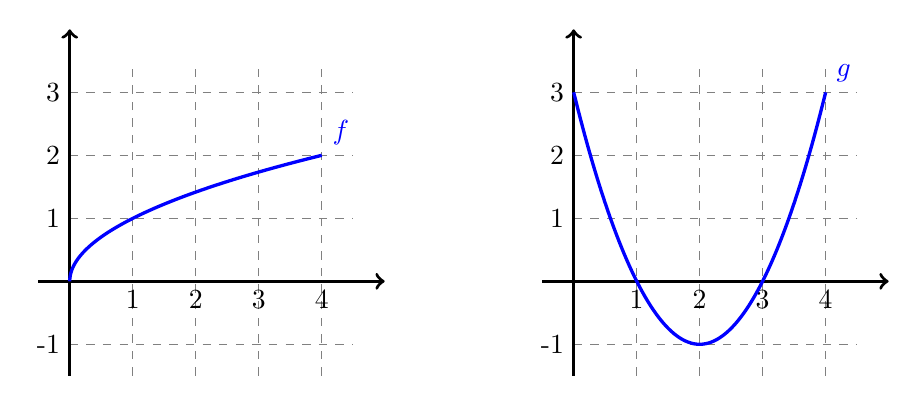
\begin{tikzpicture}[scale=0.8]
\draw[dashed, gray] (0,-1.5) grid (4.5,3.5);
\draw[very thick,->] (-0.5,0) -- (5,0);
\draw[very thick,->] (0,-1.5) -- (0,4);
\foreach \i in {1,...,4} {
  \draw (\i,0) node[below] {\i};
}
\foreach \i in {-1,1,2,3} {
  \draw (0,\i) node[left] {\i};
}
\draw[rotate = 90,very thick, blue] (0,0) parabola bend (0,0) (2,-4) node[above right] {$f$};
\begin{scope}[xshift=8cm]
\draw[dashed, gray] (0,-1.5) grid (4.5,3.5);
\draw[very thick,->] (-0.5,0) -- (5,0);
\draw[very thick,->] (0,-1.5) -- (0,4);
\foreach \i in {1,...,4} {
  \draw (\i,0) node[below] {\i};
}
\foreach \i in {-1,1,2,3} {
  \draw (0,\i) node[left] {\i};
}
\draw[very thick, blue] (0,3) parabola bend (2,-1) (4,3) node[above right] {$g$};
\end{scope}
\end{tikzpicture}
\end{center}

Use the graphs to evaluate $g(f(4))$ and $f(g(1))$. 
\vfill

\item Sketch a graph of the function $f(x) = 4-(x+1)^2$ by plotting the y-values at $x = 0$, $\pm 1$, and $\pm 2$ and then filling in the rest of the graph. 
\vfill
\vfill
\vfill

\newpage
\item The amount of garbage produced by a city (measured in tons per week) is given by a function $g(p)$ where the variable $p$ is the city's population measured in thousands of people.  One city has a population of 40,000 people and produces 13 tons of garbage each week.  In function notation, this would be expressed as (fill in the blanks): 

{\LARGE
$$ g( \hspace{0.7in} ) = {\hspace*{1in}}$$ 
}

\item The inverse of the function $g$ in the last problem would be written $g^{-1}$. Explain what the information $g^{-1}(5) = 18$ would tell us about a city. That is, what is its population and garbage production? 
\vfill

\item Suppose that $f(x)$ is a linear function such that $3 =f(0)$ and $5 = f(1)$. Find the formula for $f(x)$. 
\vfill

\item If $f(x) = 3x+1$, then what is $f(f(x))$? Simplify your answer.  
\vfill


%\item Compute the inverse of the function $f(x) = \sqrt{x+4}$. 
%\vfill
%\vfill
%\vfill


\item The time in seconds that it takes a pendulum to complete a full oscillation (swing back and forth) is $T = 2 \pi \sqrt{\dfrac{L}{9.8}}$ where $L$ is the length of the pendulum in meters.  Find the inverse of this function.  
\vfill 

\item The function $A(r) = \pi r^2$ computes the area of a circle of radius $r$. Find the formula for the inverse function and describe in words what it computes about a circle.
\vfill

\item What is the domain of the function $h(x) = \sqrt{6-x}$? That is, what $x$-values make sense as inputs?
\vfill


\setcounter{enumCount}{\theenumi}
\end{enumerate}

\newpage

\begin{enumerate}
\setcounter{enumi}{\theenumCount}

\item Use the graph below to find the values of $x$ for which $f(x) = x^{3} - 13 x + 12 > 0.$ 

\begin{flushright}
\begin{tikzpicture}[scale=0.6]
%\draw[black!50,very thin] (-3.2,-1.7) grid (3.2,1.7);
\draw[very thick,<->] (-5.3,0) -- (5.3,0) node[below] {$x$};
\draw[very thick,<->] (0,-1.8) -- (0,3.3) node[left] {$y$};
\draw[very thick,color=blue,<->] plot[domain=-4.3:4.1,samples=400] function {(x**3 - 13*x+12)/10};
\draw (-4,0.2) -- (-4,-0.2) node[below] {$-4$};
\draw  (1,0.2) -- (1,-0.2) node[below] {$1$};
\draw  (3,0.2) -- (3,-0.2) node[below] {$3$};
\draw (3.25,3) node[blue] {$f(x)$};
\end{tikzpicture}
\end{flushright}

\setcounter{enumCount}{\theenumi}
\end{enumerate}


\begin{enumerate}
\setcounter{enumi}{\theenumCount}
\item A bakery sells cupcakes.  If they gave away cupcakes for free, people would demand 1200 cupcakes per day.  For every dollar the price of a cupcake increases above 0, they will sell 200 fewer cupcakes per day.  Find a formula for the quantity of cupcakes $Q(p)$ they will sell as a function of the price $p$ of a cupcake in dollars. \vfill

\item Find the total revenue $R(p)$ that the bakery in the previous problem will earn selling cupcakes as a function of $p$. Recall that revenue is price times quantity sold.  \vfill



\setcounter{enumCount}{\theenumi}
\end{enumerate}

\noindent
A store can produce souvenir T-shirts at a cost of \$2 each. They need to choose a price for the shirts. If they sell the shirts for \$5 each, they will sell $4,000$ shirts.  If they raise the price, then for each \$1 increase in price, 400 fewer shirts will be sold.  Using the variable $p$ to represent the price that the store charges, find each of the following functions:

\begin{enumerate}
\setcounter{enumi}{\theenumCount}
\item Quantity of shirts sold: $Q(p)$ 
\vfill

\item Revenue (total money they get from selling shirts): $R(p)$  \vfill

\item Cost (total money they spend to make the shirts): $C(p)$ \vfill

\item Profit (revenue minus cost): $P(p)$  \vfill


\setcounter{enumCount}{\theenumi}
\end{enumerate}

\end{document}
